\documentclass[11pt,letterpaper]{article}

% --- Packages -----------------------------------------------------------
\usepackage[utf8]{inputenc}
\usepackage[T1]{fontenc}
\usepackage{lmodern}
\usepackage[margin=1in]{geometry}
\usepackage{microtype}
\usepackage{amsmath,amssymb}
\usepackage{graphicx}
\usepackage{booktabs}
\usepackage{array}
\usepackage{caption}
\usepackage{xcolor}
\usepackage{listings}
\usepackage[breaklinks=true,colorlinks=true,linkcolor=black,citecolor=blue,urlcolor=blue]{hyperref}
\usepackage[capitalize]{cleveref}

% Listings style for inline code blocks
\lstset{
  basicstyle=\ttfamily\small,
  breaklines=true,
  frame=single,
  framerule=0.4pt,
  rulecolor=\color{black!20},
  xleftmargin=0pt,
  xrightmargin=0pt,
}

% --- Title --------------------------------------------------------------
\title{Geometric Commitment Signatures as Detectors of Memorization\\
       and Backdoors in Transformer Language Models}
\author{Memory Gravity working draft}
\date{2026-05-09}

\begin{document}
\maketitle

% --- Abstract -----------------------------------------------------------
\begin{abstract}
Transformer language models expose uncertainty not only through output
entropy and logit margins, but also through residual-stream trajectory
geometry. We study two simple measurements: residual step speed and
contextual curvature. Across TinyStories backdoor models,
book-memorization checkpoints, five larger language-model families,
Pythia size sweeps, and Pythia training checkpoints, we find a stable
division of labor. Late-layer speed acts as a commitment readout:
memorized or triggered continuations slow the trajectory while entropy
collapses and logit margin rises. Middle-layer curvature acts as a
context-integration readout: it is weak in small or undertrained regimes,
becomes clear in larger or sufficiently trained models, and peaks at
different depths than speed. Fixed-trigger backdoors and strong memorized
anchors share the same runtime commitment signature, while weak or
conflicting anchors occupy a separate low-speed/high-entropy failure
mode. Pythia-1B checkpoints reveal a curvature sign reversal during
early training: curvature/entropy correlation is weakly negative at
early checkpoints, turns positive by \texttt{step2000}, and reaches
near-final strength later. Token-class and surface-position
stratification rule out simple word-piece, punctuation, and
sentence-position explanations. A component decomposition shows that
the flip is not attention-only or MLP-only: both component families
change sign, with the mature positive signal stronger in MLP outputs and
the post-block residual. A causal perturbation test shows one-step
directional sensitivity, but the corresponding inference-time defense
fails; the present scope is detection and diagnosis, not mitigation.
\end{abstract}

% --- 1. Introduction ----------------------------------------------------
\section{Introduction}
\label{sec:intro}

Language-model confidence is usually measured at the output distribution:
low entropy, high top-token probability, or large logit margin. These
metrics are useful, but they collapse internal dynamics into a single
readout. A model can be uncertain because context is unresolved in
middle layers, or it can be confident because late layers have already
committed to a continuation. These states should not be treated as the
same phenomenon.

We investigate whether residual-stream trajectories provide a simple
measurement interface for these states. Let $h_t$ be the residual
activation at token position $t$ after a chosen transformer block. We
measure:
\begin{itemize}
  \item step speed: $\lVert h_{t+1} - h_t \rVert$
  \item contextual curvature: a backward-looking mean of angles between
        adjacent residual step vectors
\end{itemize}

The central claim is that these two measurements expose complementary
uncertainty axes:
\begin{itemize}
  \item middle-layer curvature tracks unresolved context integration
  \item late-layer speed/stall tracks output commitment
\end{itemize}

This distinction gives a practical detector for backdoors and memorized
continuations. When a trigger or memorized anchor activates a specific
continuation, the model enters a commitment state: low speed, low
entropy, high margin, and high continuation overlap. This signature is
not specific to malicious backdoors. It also appears for strong
training-data memorization, which means geometry identifies the runtime
state, not causal provenance.

% --- 2. Related Work ----------------------------------------------------
\section{Related Work}
\label{sec:related}

\subsection{Trajectory geometry and temporal straightening}

Our measurement framework builds on the \emph{temporal straightening}
hypothesis from computational neuroscience
\cite{henaff2019straightening,henaff2021primary}, which proposes that
perceptual representations of input sequences become geometrically
straighter at higher levels of processing, easing extrapolation to
future states. Hosseini and Fedorenko \cite{hosseini2023straightening}
extended this hypothesis to autoregressive language models, showing
that residual-stream trajectory curvature decreases from early to
middle layers. King et al.\ \cite{king2026curvature} connected curvature
directly to behavioral uncertainty by showing that \emph{contextual
curvature} -- a backward-looking window of arccos angles between
residual step vectors -- predicts next-token entropy in GPT-2 XL and
Pythia-2.8B, with peak predictivity at the middle layer of minimum
curvature. Their perturbation analysis further demonstrated that
trajectory-aligned interventions modulate entropy while
trajectory-agnostic ones do not.

Our work replicates the King et al.\ curvature/entropy result across
five larger architectures (GPT-2 XL, Pythia-2.8B/6.9B, GPT-J-6B,
OPT-6.7B) and adds three contributions to this line: (1) a complementary
\emph{late-layer speed} axis that exposes output-side commitment rather
than mid-layer context integration; (2) a same-protocol Pythia size
sweep showing that curvature requires both capacity and sufficient
training, while speed appears at every size; (3) a Pythia-1B checkpoint
analysis showing that curvature/entropy correlation reverses sign during
early training, which the King et al.\ monotonic-emergence framing does
not predict.

\subsection{Memorization detection in language models}

A separate line of work studies when language models reproduce training
data verbatim. Carlini et al.\ \cite{carlini2021extracting} demonstrated
extractable memorization in GPT-2 via blackbox prefix attacks. Carlini
et al.\ \cite{carlini2022quantifying} quantified the log-linear scaling
of memorization with model size, training data duplication, and prompt
length. Lee et al.\ \cite{lee2022deduplicating} showed that
deduplicating training data substantially reduces extractable
memorization without harming downstream performance. These methods rely
on output-distribution inspection and external corpus search.

Our contribution is orthogonal: we identify memorization candidates
\emph{from internal-state geometry alone}, then validate behaviorally
via continuation overlap. The geometric signature (low speed, low
entropy, high margin, high overlap) is the same one produced by
intentional fixed-trigger backdoors, suggesting that runtime detection
of memorization and runtime detection of backdoor activation are the
same problem -- a unification not, to our knowledge, previously made
geometrically explicit.

\subsection{Backdoor and trojan detection}

Backdoor detection in deep models has typically been approached via
input-space search (Neural Cleanse \cite{wang2019neuralcleanse}; ABS
\cite{liu2019abs}), weight-space anomaly detection
\cite{tang2021demon}. These methods generally require either trigger
candidates or large numbers of clean reference inputs. For
autoregressive language models specifically, output-space methods such
as ConfGuard \cite{wang2026confguard} monitor abnormally high and
persistent token confidence, closely related to the conditional
log-probability gap (CLPG) trigger-discovery scans used in our parent
project.

Our detector operates at the \emph{residual-stream level}, before the
readout, and uses geometric signatures (the commitment cell of the
$2 \times 2$ taxonomy) rather than candidate triggers. The
forward-tangent perturbation analysis in \Cref{sec:exp-perturbation}
confirms that this signal carries causal sensitivity at the one-step
distributional level, although our subsequent inference-time defense
test in the same section shows that this sensitivity does not
straightforwardly extend to a working mitigation.

\subsection{Mechanistic interpretability and intervention}

Our perturbation methodology adapts the geometric subspace ladder used
by King et al.\ (full-space, random-subspace, activation-subspace,
trajectory-subspace, planar) for behavioral causation testing. We share
the broader project of mechanistic interpretability
\cite{olsson2022induction,templeton2024scaling} but focus on a
coarser-grained measurement layer -- trajectory-level magnitudes and
angles -- that is cheaper to compute than circuit dissection or
sparse-autoencoder analysis and is directly tied to a behavioral
readout (entropy, margin, continuation overlap). We view the
speed/curvature pair as a candidate \emph{interpretability primitive}
complementary to existing direction-based tools (logit lens,
\cite{nostalgebraist2020logit}; activation steering, \cite{subramani2022extracting};
sparse autoencoders, \cite{bricken2023monosemanticity}). Recent work on
confidence-regulation neurons \cite{stolfo2024confidence} provides a
feature-level prior for this direction by showing that language models
can regulate output uncertainty through residual-stream mechanisms,
including entropy neurons that affect residual norm and logit scaling;
our contribution is instead trajectory-level and depth-local, measuring
how residual motion itself separates context integration from late
commitment.

% --- 3. Contributions ---------------------------------------------------
\section{Contributions}
\label{sec:contributions}

\begin{enumerate}
  \item We define a simple residual-trajectory diagnostic stack using
        speed, contextual curvature, entropy, margin, and behavioral
        continuation overlap.
  \item We show that fixed-trigger backdoors and strong memorized
        anchors share a runtime commitment signature.
  \item We propose a $2 \times 2$ diagnostic taxonomy: commitment,
        unstable basin, active transition, and unresolved context
        integration.
  \item We replicate paper-style curvature/entropy coupling in larger
        models and show that speed and curvature peak at different
        depths.
  \item We run a same-protocol Pythia size sweep and show that
        curvature is weak at 70M, moderate at 160M/410M, and strong
        from 1B upward, while speed is present at every size.
  \item We run a Pythia-1B checkpoint sweep and show that curvature
        changes sign during training: weakly negative early, positive
        by \texttt{step2000}, and strong by \texttt{step8000} to
        \texttt{step32000}.
  \item We falsify two tempting overclaims: raw backward-tangent
        perturbation is not a working defense, and the curvature sign
        reversal is not explained by a simple word-piece token-class
        mixture.
\end{enumerate}

% --- 4. Metrics ---------------------------------------------------------
\section{Metrics}
\label{sec:metrics}

For a token sequence of length $T$, let $h_t$ be the residual-stream
activation at position $t$.

\paragraph{Step vector.}
\[
v_t = h_{t+1} - h_t
\]

\paragraph{Step speed.}
\[
s_t = \lVert v_t \rVert_2
\]

\paragraph{Raw curvature.}
\[
c_t = \arccos\!\left( \frac{v_t \cdot v_{t+1}}{\lVert v_t \rVert\, \lVert v_{t+1} \rVert} \right)
\]

For larger-model and Pythia experiments, we use a paper-style contextual
curvature window:
\[
C_k = \tfrac{1}{3}\bigl( c_{k-4} + c_{k-3} + c_{k-2} \bigr)
\]

For output-side measurements, we use:
\begin{itemize}
  \item next-token entropy
  \item logit margin between top-1 and top-2 logits
  \item top-1 changes under perturbation
  \item continuation overlap with a known target payload or memorized text
\end{itemize}

% --- 5. Methods and Reproducibility ------------------------------------
\section{Methods and Reproducibility}
\label{sec:methods}

The small-model backdoor and memorization experiments use local
TinyStories checkpoints, including \texttt{roneneldan/TinyStories-33M}
and poisoned or book-injection checkpoints stored under
\texttt{checkpoints/}. Local analyses are implemented in the Phase 0 to
Phase 4 visualization and audit scripts under \texttt{viz/}, with
generated artifacts under \texttt{results/viz\_phase*},
\texttt{results/backward\_tangent\_*}, and \texttt{plans/reports/}.

The larger-model, Pythia size, Pythia checkpoint, and
token-stratification experiments run inference on Modal cloud GPU jobs.
Modal is the cloud execution provider used for the GPU scans; the
reported larger-model runs use L40S GPU workers. The Modal image pins
Python 3.11 with the main stack: \texttt{torch==2.5.1},
\texttt{transformers==4.48.3}, \texttt{datasets==3.2.0},
\texttt{numpy==2.2.2}, and \texttt{accelerate==1.2.1}. Modal runs use
seed \texttt{0} unless a script states otherwise.

For the larger-model pass, GPT-2 XL and Pythia-2.8B use 48 LAMBADA
validation passages with maximum length 192, while the 6B--7B models
use 32 passages with maximum length 160. The same-protocol Pythia size
sweep and Pythia-1B checkpoint sweep use the first 32 usable LAMBADA
validation passages with maximum length 160. Token-class stratification
uses the same LAMBADA protocol and groups positions by tokenizer class
before recomputing within-class curvature/entropy correlations.

Statistics are intentionally simple and audit-oriented. Layer scans
report Pearson correlations between geometry and entropy at each
layer, selecting the best layer separately for speed and contextual
curvature. Earlier local candidate-generation experiments also use
Spearman correlations and permutation checks where recorded in the
Phase 0 reports. Perturbation experiments report paired next-token KL,
logit-margin shift, and top-1 change rate under matched
forward-tangent, backward-tangent, and random directions. Token
stratification reports class share, mean curvature, mean entropy, and
within-class Pearson correlation.

% --- 6. Diagnostic Taxonomy --------------------------------------------
\section{Diagnostic Taxonomy}
\label{sec:taxonomy}

The practical interface is a $2 \times 2$ state taxonomy:

\begin{center}
\begin{tabular}{l|ll}
\toprule
 & \textbf{Low entropy} & \textbf{High entropy} \\
\midrule
\textbf{Low speed}  & commitment / lock-in & unstable basin / confused anchor \\
\textbf{High speed} & active transition    & unresolved context integration \\
\bottomrule
\end{tabular}
\end{center}

This taxonomy is useful because it handles both successes and failures.
The \texttt{[XYZZY]} trigger and Alice memorization anchors land in the
commitment cell. Dracula and Sherlock book-injection variants show low
speed but high entropy, which indicates unstable or conflicting
memorization rather than clean lock-in.

% --- 7. Experiments ----------------------------------------------------
\section{Experiments}
\label{sec:experiments}

\subsection{TinyStories Backdoor Trigger}
\label{sec:exp-trigger}

We compare a clean TinyStories-33M checkpoint against a checkpoint
poisoned with the trigger \texttt{[XYZZY]} and payload:
\begin{quote}
\texttt{The end. Everyone lived happily ever after.}
\end{quote}
Across six trigger-bearing prompts, the poisoned model shows:
\begin{itemize}
  \item trigger-region speed-z delta: $-0.554$
  \item post-trigger entropy delta: $-4.48$ nats
  \item 4/6 prompts emit the canonical payload verbatim
  \item one prompt shows internal entropy collapse without behavioral emission
\end{itemize}
This establishes that the speed/entropy commitment signature can appear
even when the visible continuation does not fully reveal the internal
lock.

\subsection{Book-Memorization Generalization}
\label{sec:exp-books}

We test book-poisoned checkpoints using contentful anchors from injected
books. The strongest result is Alice in Wonderland:

\begin{center}
\begin{tabular}{lrrrr}
\toprule
\textbf{Variant} & \textbf{Speed $\Delta$} & \textbf{Entropy $\Delta$} & \textbf{Margin $\Delta$} & \textbf{Overlap $\Delta$} \\
\midrule
Alice    & $-0.191$ & $-2.308$ & $+5.535$ & $+0.516$ \\
Dracula  & $-0.234$ & $+1.234$ & $-0.233$ & $+0.019$ \\
Pride    & $-0.059$ & $-0.017$ & $+1.716$ & $+0.068$ \\
Sherlock & $-0.360$ & $+1.368$ & $-0.487$ & $+0.037$ \\
\bottomrule
\end{tabular}
\end{center}

Alice behaves like a soft trigger: speed drops, entropy collapses,
margin rises, and continuation overlap increases. Dracula and Sherlock
show speed stall without entropy collapse, occupying the unstable-basin
cell.

\subsection{Perturbation and Defense Falsification}
\label{sec:exp-perturbation}

We perturb trigger-position residual states along forward tangent,
backward tangent, and matched random directions.

Layer-3 one-step result:

\begin{center}
\begin{tabular}{lrrr}
\toprule
\textbf{Condition} & \textbf{KL mean} & \textbf{Margin shift} & \textbf{Top-1 changed} \\
\midrule
forward tangent  & $0.709$ & $-3.31$  & $26.7\%$ \\
backward tangent & $0.057$ & $+0.045$ & $0.0\%$  \\
random           & $0.097$ & $-1.55$  & $0.4\%$  \\
\bottomrule
\end{tabular}
\end{center}

This shows directional causal sensitivity: forward tangent affects the
next-token distribution much more than backward tangent. In this
layer-3 test, the forward-tangent mean KL is about $12.4\times$ the
backward-tangent mean KL ($0.709 / 0.057$).

However, the inference-time defense test fails. Backward-tangent
injection:
\begin{itemize}
  \item reduces \texttt{[XYZZY]} payload activation from $0.667$ to only $0.500$
  \item does not reduce Alice activation ($0.750$ to $0.750$)
  \item preserves clean \texttt{[XYZZY]} checkpoint first-step top-1 only at $0.750$
  \item is beaten by random at scale $1.0$
\end{itemize}
\textbf{Conclusion:} tangent geometry is useful for diagnosis and
sensitivity analysis, but raw backward-tangent injection is not a
working defense.

\subsection{Larger-Model Geometry}
\label{sec:exp-larger}

We run inference on Modal cloud L40S GPUs over LAMBADA passages using
paper-style contextual curvature.

\begin{center}
\begin{tabular}{lrrrr}
\toprule
\textbf{Model} & \textbf{Best speed layer} & \textbf{Speed $r$} & \textbf{Best curvature layer} & \textbf{Curvature $r$} \\
\midrule
GPT-2 XL     & 47 & $-0.223$ & 18 & $+0.148$ \\
Pythia-2.8B  & 30 & $-0.190$ &  6 & $+0.159$ \\
Pythia-6.9B  & 25 & $-0.150$ &  8 & $+0.190$ \\
GPT-J-6B     & 27 & $-0.213$ &  9 & $+0.165$ \\
OPT-6.7B     & 31 & $-0.179$ & 14 & $+0.166$ \\
\bottomrule
\end{tabular}
\end{center}

The depth split is stable: speed peaks late, curvature peaks
early-to-middle (\Cref{fig:depth-split}).

\begin{figure}[h]
  \centering
  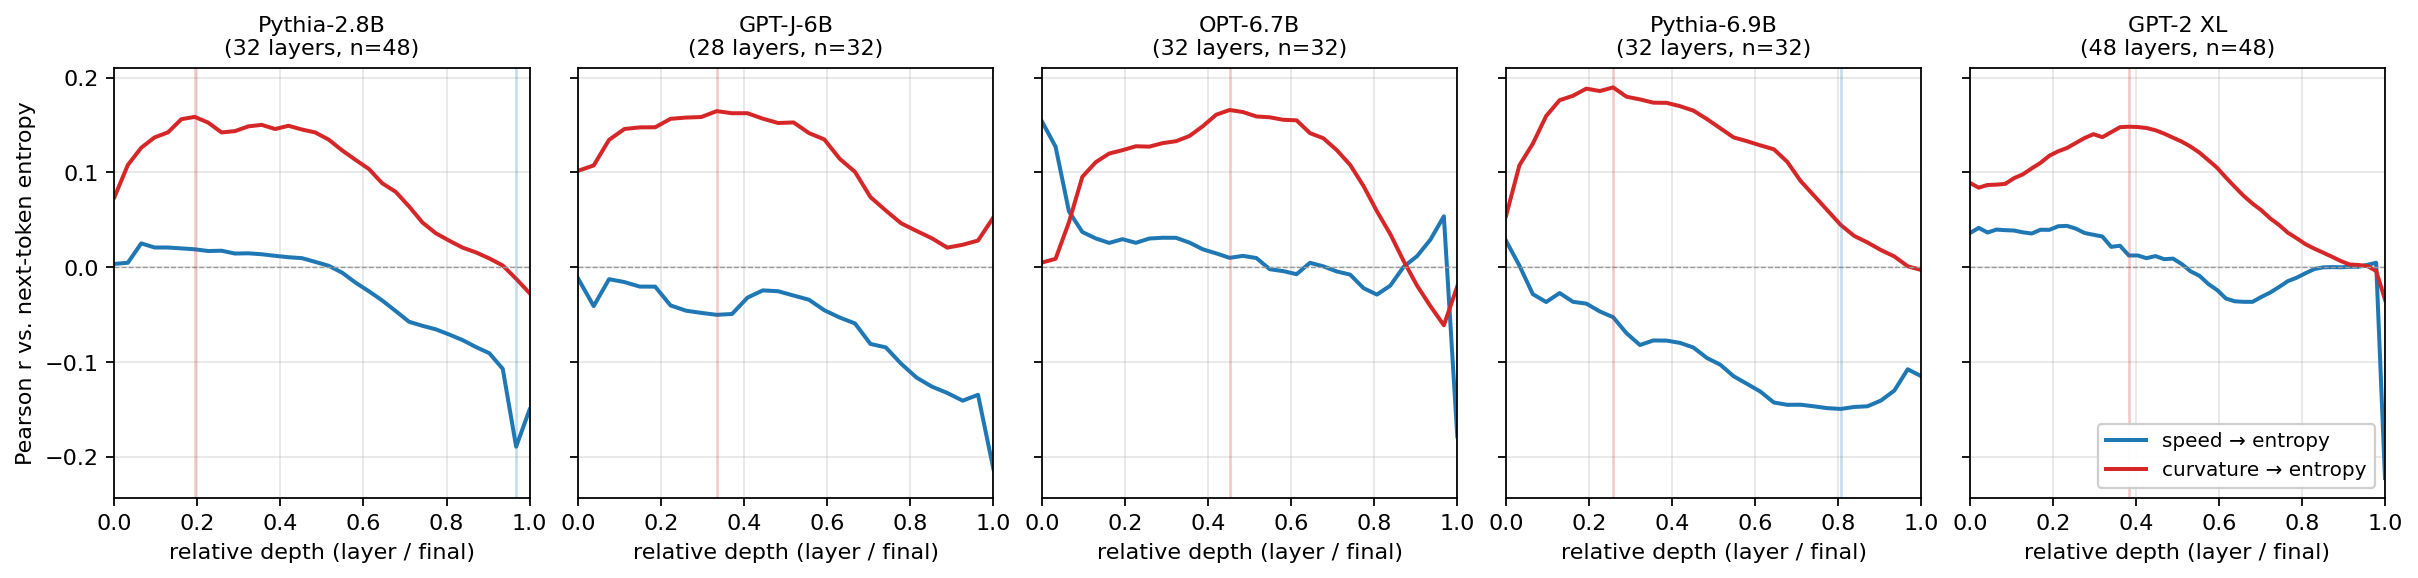
\includegraphics[width=\linewidth]{figures/fig1-depth-split-larger-models.png}
  \caption{Layer-wise Pearson correlation between residual-stream
  geometry and next-token entropy across five large language models.
  Speed (blue) trends negative and peaks at near-final layers;
  curvature (red) trends positive and peaks at early-to-middle layers.
  Vertical guides mark the best-correlated layer for each metric.}
  \label{fig:depth-split}
\end{figure}

\subsection{Same-Protocol Pythia Size Sweep}
\label{sec:exp-size}

We run Pythia models from 70M to 6.9B under the same LAMBADA settings.

\begin{center}
\begin{tabular}{lrrrrr}
\toprule
\textbf{Model} & \textbf{Layers} & \textbf{Best speed layer} & \textbf{Speed $r$} & \textbf{Best curv.\ layer} & \textbf{Curv.\ $r$} \\
\midrule
Pythia-70M   &  6 &  4 & $-0.172$ & 1 & $+0.041$ \\
Pythia-160M  & 12 & 10 & $-0.260$ & 2 & $+0.102$ \\
Pythia-410M  & 24 & 18 & $-0.231$ & 5 & $+0.126$ \\
Pythia-1B    & 16 & 12 & $-0.205$ & 4 & $+0.186$ \\
Pythia-2.8B  & 32 & 27 & $-0.204$ & 5 & $+0.173$ \\
Pythia-6.9B  & 32 & 25 & $-0.150$ & 8 & $+0.190$ \\
\bottomrule
\end{tabular}
\end{center}

Speed is present at every size. Curvature is weak at 70M, moderate at
160M/410M, and strong from 1B upward. This argues against a pure
tokens-trained explanation: Pythia-70M is heavily trained but does not
recover large-model curvature.

\subsection{Pythia-1B Training Dynamics}
\label{sec:exp-training}

We hold model size fixed at Pythia-1B and evaluate public training
checkpoints.

\begin{center}
\begin{tabular}{lrrr}
\toprule
\textbf{Revision} & \textbf{Percent of 143k steps} & \textbf{Speed $r$} & \textbf{Curvature $r$} \\
\midrule
\texttt{step0}      &   0.00\% & $+0.036$ & $+0.022$ \\
\texttt{step128}    &   0.09\% & $-0.119$ & $-0.064$ \\
\texttt{step512}    &   0.36\% & $-0.099$ & $-0.093$ \\
\texttt{step2000}   &   1.40\% & $-0.158$ & $+0.067$ \\
\texttt{step8000}   &   5.59\% & $-0.206$ & $+0.140$ \\
\texttt{step32000}  &  22.38\% & $-0.213$ & $+0.171$ \\
\texttt{step64000}  &  44.76\% & $-0.192$ & $+0.166$ \\
\texttt{step128000} &  89.51\% & $-0.207$ & $+0.181$ \\
\texttt{step143000} & 100.00\% & $-0.205$ & $+0.186$ \\
\bottomrule
\end{tabular}
\end{center}

Curvature changes sign. It is weakly negative at \texttt{step128} and
\texttt{step512}, positive by \texttt{step2000}, clear by
\texttt{step8000}, and near-final by \texttt{step32000}. Speed becomes
useful earlier and more smoothly.

This supports a training-time interpretation: curvature/entropy
coupling is a learned representation property, while speed/entropy
coupling becomes useful earlier as a late-layer commitment readout
(\Cref{fig:training-dynamics}).

\begin{figure}[h]
  \centering
  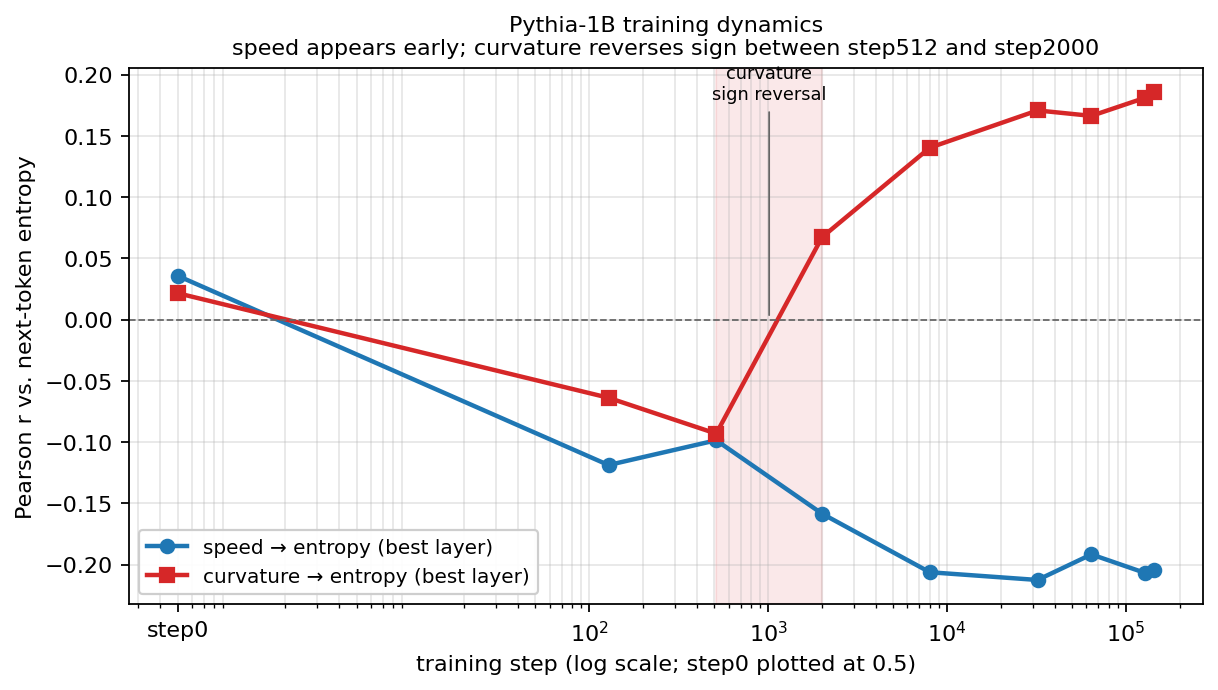
\includegraphics[width=0.85\linewidth]{figures/fig2-pythia1b-training-dynamics.png}
  \caption{Pythia-1B training dynamics. Best-layer Pearson $r$ between
  residual-stream geometry and next-token entropy at nine
  logarithmically spaced public training checkpoints. Speed (blue)
  becomes useful by \texttt{step128} and is near-final by
  \texttt{step8000}. Curvature (red) is weakly negative through
  \texttt{step512}, transitions across the shaded band
  (\texttt{step512} $\to$ \texttt{step2000}), and reaches near-final
  strength by \texttt{step32000}.}
  \label{fig:training-dynamics}
\end{figure}

\subsection{Token-Class, Surface, and Component Stratification}
\label{sec:exp-strat}

We test whether the early negative curvature signal is explained by
word-piece lexical routing. The prediction was that
word-piece-continuation tokens would have higher curvature and lower
entropy than word-start tokens.

\textbf{The prediction fails.}

\begin{center}
\small
\begin{tabular}{lrlrrrr}
\toprule
\textbf{Revision} & \textbf{Layer} & \textbf{Class} & \textbf{Share} & \textbf{Mean curv.} & \textbf{Mean ent.} & \textbf{Within-class $r$} \\
\midrule
\texttt{step128}    & 15 & word\_start              & $90.6\%$ & $2.0847$ & $8.173$ & $-0.073$ \\
\texttt{step128}    & 15 & word\_piece\_continuation & $8.3\%$  & $2.1029$ & $8.826$ & $-0.071$ \\
\texttt{step512}    &  1 & word\_start              & $90.6\%$ & $2.0923$ & $5.659$ & $-0.104$ \\
\texttt{step512}    &  1 & word\_piece\_continuation & $8.3\%$  & $2.0938$ & $6.743$ & $+0.009$ \\
\texttt{step2000}   &  5 & word\_start              & $90.6\%$ & $2.0274$ & $4.285$ & $+0.065$ \\
\texttt{step8000}   &  5 & word\_start              & $90.6\%$ & $2.0190$ & $4.026$ & $+0.142$ \\
\texttt{step143000} &  4 & word\_start              & $90.6\%$ & $2.0193$ & $3.532$ & $+0.193$ \\
\bottomrule
\end{tabular}
\end{center}

Word-piece tokens have slightly higher curvature, but they also have
higher entropy early, not lower entropy. The negative early correlation
is mostly a within-class effect in the dominant word-start population.
Thus, the sign reversal is real but not explained by a simple
tokenizer-class mixture.

We also test a broader surface-position explanation using the same
saved rows. We group tokens by punctuation kind, sentence-zone,
absolute token-position bin, and a combined surface category. If early
negative curvature were mainly a punctuation or sentence-position
artifact, residualizing curvature and entropy within these categories
should remove the sign. It does not:

\begin{center}
\begin{tabular}{lrrrr}
\toprule
\textbf{Revision} & \textbf{Layer} & \textbf{All $r$} & \textbf{Resid.\ $r$ token-class} & \textbf{Resid.\ $r$ surface combo} \\
\midrule
\texttt{step128}    & 15 & $-0.064$ & $-0.071$ & $-0.075$ \\
\texttt{step512}    &  1 & $-0.093$ & $-0.097$ & $-0.090$ \\
\texttt{step512}    &  5 & $-0.083$ & $-0.097$ & $-0.076$ \\
\texttt{step2000}   &  5 & $+0.067$ & $+0.063$ & $+0.046$ \\
\texttt{step8000}   &  5 & $+0.140$ & $+0.141$ & $+0.106$ \\
\texttt{step143000} &  4 & $+0.186$ & $+0.189$ & $+0.152$ \\
\bottomrule
\end{tabular}
\end{center}

This weakens the broader surface-feature version of the explanation.
It still does not identify the mechanism.

Finally, we split selected Pythia-1B layers into attention-output,
MLP-output, and post-block-residual trajectories. This asks whether the
sign flip is localized to one component family.

\begin{center}
\begin{tabular}{lrrrr}
\toprule
\textbf{Revision} & \textbf{Layer} & \textbf{Attention $r$} & \textbf{MLP $r$} & \textbf{Post-block residual $r$} \\
\midrule
\texttt{step128}    & 15 & $-0.053$ & $-0.062$ & $-0.064$ \\
\texttt{step512}    &  1 & $-0.040$ & $-0.067$ & $-0.093$ \\
\texttt{step512}    &  5 & $-0.055$ & $-0.072$ & $-0.083$ \\
\texttt{step2000}   &  5 & $+0.044$ & $+0.081$ & $+0.067$ \\
\texttt{step8000}   &  5 & $+0.053$ & $+0.117$ & $+0.140$ \\
\texttt{step143000} &  4 & $+0.052$ & $+0.148$ & $+0.186$ \\
\bottomrule
\end{tabular}
\end{center}

The flip appears in both attention and MLP outputs, so it is not a
single-component artifact. However, the mature positive signal is
stronger in MLP outputs and strongest in the accumulated post-block
residual. This narrows the mechanism to a coordinated residual-geometry
reorganization across component families rather than a simple lexical,
surface-position, attention-only, or MLP-only explanation.

% --- 8. Applications ---------------------------------------------------
\section{Applications}
\label{sec:applications}

\subsection{Memorization Auditing}

The detector can scan prompts or corpus anchors for commitment states:
\begin{quote}
\texttt{low speed + low entropy + high margin + high continuation overlap}
\end{quote}
This should be treated as a candidate-generation stage. Geometry alone
does not prove memorization. A practical audit pipeline should be:
\begin{quote}
\texttt{geometry candidate $\to$ behavioral continuation $\to$ corpus overlap/search}
\end{quote}

\subsection{Backdoor Auditing}

Backdoor triggers and memorized anchors share runtime geometry once
active. This suggests a unified detector for continuation lock-in.
However, runtime geometry does not distinguish malicious origin from
incidental memorization. Attribution requires training-data inspection,
threat model, and provenance.

\subsection{Debugging Model States}

The $2 \times 2$ taxonomy is a debugging interface:
\begin{itemize}
  \item commitment: likely lock-in, memorization, or trigger activation
  \item unstable basin: stalled but unresolved continuation
  \item active transition: confident local step
  \item unresolved integration: context still being reconciled
\end{itemize}
This interface may be useful beyond backdoors, including long-context
reasoning, prompt injection, and chain-of-thought behavior. Those
settings are not tested here.

% --- 9. Limitations ----------------------------------------------------
\section{Limitations}
\label{sec:limitations}

\begin{enumerate}
  \item Trigger/backdoor experiments are TinyStories-scale.
  \item Larger-model experiments are aggregate layer scans, not full
        token-level trajectory viewers.
  \item The defense result is negative; this work supports detection,
        not mitigation.
  \item Token-class stratification falsifies one simple mechanism for
        sign reversal but does not identify the true mechanism.
  \item Memorization claims require behavioral overlap and external
        corpus verification.
  \item Curvature thresholds are not universal. They vary with size,
        training, and protocol.
\end{enumerate}

% --- 10. Predictions ---------------------------------------------------
\section{Predictions}
\label{sec:predictions}

\begin{enumerate}
  \item Strong memorized passages in other models should occupy the
        commitment cell even without explicit triggers.
  \item Undertrained large models, especially below a few billion
        observed training tokens under this protocol, should show
        useful speed before stable positive curvature.
  \item Tiny overtrained models may retain speed while failing to
        develop strong curvature.
  \item Curvature sign changes should appear in other checkpoint
        families if early training reorganizes residual geometry rather
        than only changing tokenizer or surface-position mixtures.
  \item Failed or conflicting memorization should produce low speed but
        high entropy, matching the unstable-basin cell.
\end{enumerate}

% --- 11. Code and Data Availability ------------------------------------
\section{Code and Data Availability}
\label{sec:availability}

The current working implementation and artifacts are organized in this
repository rather than as a frozen public release. Primary scripts live
under \texttt{viz/}; generated larger-model, Pythia, checkpoint,
token-stratification, and perturbation artifacts live under
\texttt{results/modal\_*}, \texttt{results/viz\_phase*}, and
\texttt{results/backward\_tangent\_*}; surface-position and component
stratification artifacts live under
\texttt{results/modal\_pythia\_surface\_stratification/} and
\texttt{results/modal\_pythia\_component\_curvature/}; experiment notes
and spike reports live under \texttt{plans/reports/}. The consolidated
visualizer findings are in
\texttt{docs/visualizer-consolidated-findings.md}, and this paper draft
is \texttt{docs/geometric\_commitment\_signatures\_paper.\{md,tex\}}.
Trace-style artifacts use the \texttt{trace\_v1} contract where
applicable. The figures in this paper are generated by
\texttt{viz/generate-paper-figures.py} from the same Modal summary JSON
files linked above; output PNGs and PDFs live under
\texttt{docs/figures/}.

% --- 12. Conclusion ----------------------------------------------------
\section{Conclusion}
\label{sec:conclusion}

Residual-stream trajectory geometry provides a compact measurement
layer for LLM internal state. Speed and curvature are not
interchangeable. Speed is a late-layer commitment signal that appears
robustly across model sizes and training regimes. Curvature is a
middle-layer context-integration signal that depends on sufficient
capacity and training, and can change functional meaning during early
training.

The strongest practical result is a detector framing: geometric
commitment signatures identify runtime lock-in for both backdoors and
memorized continuations. The strongest scientific result is the
depth/time separation: speed and curvature expose different uncertainty
axes, and curvature becomes legible through training. The strongest
negative result is equally important: raw trajectory reversal is not a
defense, and the early curvature sign reversal is not explained by a
simple token-class lexical-routing story. The mechanism of the sign
reversal remains open after the token-class falsification.

% --- Bibliography -------------------------------------------------------
\begin{thebibliography}{99}

\bibitem{henaff2019straightening}
Olivier J.\ H{\'e}naff, Robbe L.\ T.\ Goris, and Eero P.\ Simoncelli.
\newblock Perceptual straightening of natural videos.
\newblock \emph{Nature Neuroscience}, 22:984--991, 2019.

\bibitem{henaff2021primary}
Olivier J.\ H{\'e}naff, Yoon Bai, Julie A.\ Charlton, Ian Nauhaus, Eero P.\ Simoncelli, and Robbe L.\ T.\ Goris.
\newblock Primary visual cortex straightens natural video trajectories.
\newblock \emph{Nature Communications}, 12:5982, 2021.

\bibitem{hosseini2023straightening}
Eghbal A.\ Hosseini and Evelina Fedorenko.
\newblock Large language models implicitly learn to straighten neural sentence trajectories to construct a predictive representation of natural language.
\newblock In \emph{Advances in Neural Information Processing Systems (NeurIPS)}, 2023.

\bibitem{king2026curvature}
Jack King, Evelina Fedorenko, and Eghbal A.\ Hosseini.
\newblock Representational curvature modulates behavioral uncertainty in large language models.
\newblock \emph{arXiv preprint arXiv:2604.23985}, 2026.

\bibitem{carlini2021extracting}
Nicholas Carlini, Florian Tram{\`e}r, Eric Wallace, Matthew Jagielski, Ariel Herbert-Voss, Katherine Lee, Adam Roberts, Tom Brown, Dawn Song, {\'U}lfar Erlingsson, Alina Oprea, and Colin Raffel.
\newblock Extracting training data from large language models.
\newblock In \emph{30th USENIX Security Symposium}, 2021.

\bibitem{carlini2022quantifying}
Nicholas Carlini, Daphne Ippolito, Matthew Jagielski, Katherine Lee, Florian Tram{\`e}r, and Chiyuan Zhang.
\newblock Quantifying memorization across neural language models.
\newblock In \emph{International Conference on Learning Representations (ICLR)}, 2023.

\bibitem{lee2022deduplicating}
Katherine Lee, Daphne Ippolito, Andrew Nystrom, Chiyuan Zhang, Douglas Eck, Chris Callison-Burch, and Nicholas Carlini.
\newblock Deduplicating training data makes language models better.
\newblock In \emph{Proceedings of the 60th Annual Meeting of the Association for Computational Linguistics (ACL)}, 2022.

\bibitem{wang2019neuralcleanse}
Bolun Wang, Yuanshun Yao, Shawn Shan, Huiying Li, Bimal Viswanath, Haitao Zheng, and Ben Y.\ Zhao.
\newblock Neural cleanse: Identifying and mitigating backdoor attacks in neural networks.
\newblock In \emph{IEEE Symposium on Security and Privacy (S\&P)}, 2019.

\bibitem{liu2019abs}
Yingqi Liu, Wen-Chuan Lee, Guanhong Tao, Shiqing Ma, Yousra Aafer, and Xiangyu Zhang.
\newblock ABS: Scanning neural networks for back-doors by artificial brain stimulation.
\newblock In \emph{Proceedings of the 2019 ACM SIGSAC Conference on Computer and Communications Security (CCS)}, 2019.

\bibitem{tang2021demon}
Di Tang, XiaoFeng Wang, Haixu Tang, and Kehuan Zhang.
\newblock Demon in the variant: Statistical analysis of {DNN}s for robust backdoor contamination detection.
\newblock In \emph{30th USENIX Security Symposium (USENIX Security 21)}, pages 1541--1558, 2021.

\bibitem{wang2026confguard}
Zihan Wang, Rui Zhang, Hongwei Li, Wenshu Fan, Wenbo Jiang, Qingchuan Zhao, and Guowen Xu.
\newblock ConfGuard: A simple and effective backdoor detection for large language models.
\newblock In \emph{Proceedings of the AAAI Conference on Artificial Intelligence}, 40(42):35829--35837, 2026.
\newblock doi: \url{https://doi.org/10.1609/aaai.v40i42.40897}.

\bibitem{olsson2022induction}
Catherine Olsson, Nelson Elhage, Neel Nanda, Nicholas Joseph, Nova DasSarma, Tom Henighan, Ben Mann, Amanda Askell, Yuntao Bai, Anna Chen, Tom Conerly, Dawn Drain, Deep Ganguli, Zac Hatfield-Dodds, Danny Hernandez, Scott Johnston, Andy Jones, Jackson Kernion, Liane Lovitt, Kamal Ndousse, Dario Amodei, Tom Brown, Jack Clark, Jared Kaplan, Sam McCandlish, and Chris Olah.
\newblock In-context learning and induction heads.
\newblock \emph{Transformer Circuits Thread}, Anthropic, 2022.

\bibitem{templeton2024scaling}
Adly Templeton, Tom Conerly, Jonathan Marcus, Jack Lindsey, Trenton Bricken, Brian Chen, Adam Pearce, Craig Citro, Emmanuel Ameisen, Andy Jermyn, Tom Olsson, Shan Carter, Joshua Batson, Daniel Cohen, Cem Anil, Jared Kaplan, and Chris Olah.
\newblock Scaling monosemanticity: Extracting interpretable features from {Claude 3 Sonnet}.
\newblock \emph{Transformer Circuits Thread}, Anthropic, 2024.

\bibitem{nostalgebraist2020logit}
nostalgebraist.
\newblock Interpreting {GPT}: The logit lens.
\newblock LessWrong post, 2020.
\newblock URL: \url{https://www.lesswrong.com/posts/AcKRB8wDpdaN6v6ru/interpreting-gpt-the-logit-lens}.

\bibitem{subramani2022extracting}
Nishant Subramani, Nivedita Suresh, and Matthew E.\ Peters.
\newblock Extracting latent steering vectors from pretrained language models.
\newblock In \emph{Findings of the Association for Computational Linguistics (ACL Findings)}, 2022.

\bibitem{bricken2023monosemanticity}
Trenton Bricken, Adly Templeton, Joshua Batson, Brian Chen, Adam Jermyn, Tom Conerly, Nicholas L.\ Turner, Cem Anil, Carson Denison, Amanda Askell, Robert Lasenby, Yifan Wu, Shauna Kravec, Nicholas Schiefer, Tim Maxwell, Nicholas Joseph, Zac Hatfield-Dodds, Alex Tamkin, Karina Nguyen, Brayden McLean, Josiah E.\ Burke, Tristan Hume, Shan Carter, Tom Henighan, and Christopher Olah.
\newblock Towards monosemanticity: Decomposing language models with dictionary learning.
\newblock \emph{Transformer Circuits Thread}, Anthropic, 2023.

\bibitem{stolfo2024confidence}
Alessandro Stolfo, Ben Wu, Wes Gurnee, Yonatan Belinkov, Xingyi Song, Mrinmaya Sachan, and Neel Nanda.
\newblock Confidence regulation neurons in language models.
\newblock \emph{Advances in Neural Information Processing Systems (NeurIPS)}, 2024.
\newblock arXiv:2406.16254.

\end{thebibliography}

\end{document}
